In this section, the Server Layer is described in some detail in terms of its specific subsystems.

\subsection{PHP Scripts and Interfaces}
This section should be a general description of a particular subsystem for the given layer. For most subsystems, an extract of the architectural block diagram with data flows is useful. This should consist of the subsystem being described and those subsystems with which it communicates. 

Sript Subsystem is a portion of every .php file on the website. This data flows from HTML pages into the PHP scripts which use the information in SQL statements to retrieve or send data to the database. Then, PHP generates code for HTML output.


\begin{figure}[h!]
	\centering
 	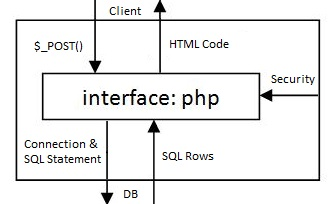
\includegraphics[width=0.60\textwidth]{images/PHPScriptSubsystem}
 \caption{PHP Script echos table formatting}
\end{figure}

\subsubsection{Assumptions}
No Assumptions were made.

\subsubsection{Responsibilities}
The PHP script is the backbone of the website. It is hosted on a internet client with access to running PHP scripts. PHP provides a means to communicate with the database and send information to client systems. Each GUI system has a backend PHP interface to display features - such as tables, user information, and create data - which pulls or pushes data to the database.

\subsubsection{Subsystem Interfaces}

\begin {table}[H]
\caption {Subsystem interfaces} 
\begin{center}
    \begin{tabular}{ | p{1cm} | p{6cm} | p{3cm} | p{3cm} |}
    \hline
    ID & Description & Inputs & Outputs \\ \hline
    \#1 & MySQL & \pbox{3cm}{SQL statement \\ Connection Data} & \pbox{3cm}{SQL Rows}  \\ \hline
    \#2 & $_POST() & _GET() & \pbox{3cm}{N/A} & \pbox{3cm}{PlainText Variable}  \\ \hline
    \#3 & echo & \pbox{3cm}{String variable} & \pbox{3cm}{HTML Code}  \\ \hline
    \end{tabular}
\end{center}
\end{table}

\subsection{Static File Storage}
The website's storage system. Internet host stores code, script and image files to be used on the website. 

\begin{figure}[h!]
	\centering
 	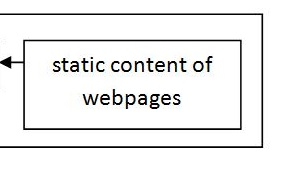
\includegraphics[width=0.60\textwidth]{images/FileStorageSubsystem}
 \caption{The File Browser Layout}
\end{figure}

\subsubsection{Assumptions}
No assumptions where made for file storage.

\subsubsection{Responsibilities}
The responsibility of the file storage is to store scripts, style, html, and security files.


\subsubsection{Subsystem Interfaces}
No system interfaces for file storage.
